%%%%%%%%%%%%%%%%%%%%%%%%%%%%%%%%%%%%%%%%%
% Journal Article
% LaTeX Template
% Version 1.4 (15/5/16)
%
% This template has been downloaded from:
% http://www.LaTeXTemplates.com
%
% Original author:
% Frits Wenneker (http://www.howtotex.com) with extensive modifications by
% Vel (vel@LaTeXTemplates.com)
%
% License:
% CC BY-NC-SA 3.0 (http://creativecommons.org/licenses/by-nc-sa/3.0/)
%
%%%%%%%%%%%%%%%%%%%%%%%%%%%%%%%%%%%%%%%%%

%----------------------------------------------------------------------------------------
%	PACKAGES AND OTHER DOCUMENT CONFIGURATIONS
%----------------------------------------------------------------------------------------

%\documentclass{article}
%\documentclass[oneside,twocolumn]{article}
\documentclass[oneside,onecolumn]{article}

\usepackage{blindtext} % Package to generate dummy text throughout this template 
\usepackage{multicol}
\usepackage[sc]{mathpazo} % Use the Palatino font
\usepackage[T1]{fontenc} % Use 8-bit encoding that has 256 glyphs
\linespread{1.05} % Line spacing - Palatino needs more space between lines
\usepackage{microtype} % Slightly tweak font spacing for aesthetics

%\usepackage[english]{babel} % Language hyphenation and typographical rules
\usepackage[spanish]{babel}
\usepackage[hmarginratio=1:1,top=32mm,columnsep=20pt]{geometry} % Document margins
\usepackage[hang, small,labelfont=bf,up,textfont=it,up]{caption} % Custom captions under/above floats in tables or figures
\usepackage{booktabs} % Horizontal rules in tables

\usepackage{lettrine} % The lettrine is the first enlarged letter at the beginning of the text

\usepackage{listings} % Required for insertion of code

\usepackage{enumitem} % Customized lists
\setlist[itemize]{noitemsep} % Make itemize lists more compact

\usepackage{abstract} % Allows abstract customization
\renewcommand{\abstractnamefont}{\normalfont\bfseries} % Set the "Abstract" text to bold
\renewcommand{\abstracttextfont}{\normalfont\small\itshape} % Set the abstract itself to small italic text

\usepackage{titlesec} % Allows customization of titles
\renewcommand\thesection{\Roman{section}} % Roman numerals for the sections
\renewcommand\thesubsection{\roman{subsection}} % roman numerals for subsections
\titleformat{\section}[block]{\large\scshape\centering}{\thesection.}{1em}{} % Change the look of the section titles
\titleformat{\subsection}[block]{\large}{\thesubsection.}{1em}{} % Change the look of the section titles

\usepackage{fancyhdr} % Headers and footers
\pagestyle{fancy} % All pages have headers and footers
\fancyhead{} % Blank out the default header
\fancyfoot{} % Blank out the default footer
%\fancyhead[C]{Running title $\bullet$ May 2016 $\bullet$ Vol. XXI, No. 1} % Custom header text
\fancyfoot[RO,LE]{\thepage} % Custom footer text

\usepackage{titling} % Customizing the title section

\usepackage{hyperref} % For hyperlinks in the PDF

\usepackage{listings}
\usepackage{algorithm2e}
\usepackage{graphicx}
\usepackage[dvipsnames]{xcolor}
\definecolor{codegreen}{rgb}{0,0.6,0}
\definecolor{codegray}{rgb}{0.5,0.5,0.5}
\definecolor{codepurple}{rgb}{0.58,0,0.82}
\definecolor{backcolour}{rgb}{1,1,1}
\lstdefinestyle{mystyle}{
    backgroundcolor=\color{backcolour},   
    commentstyle=\color{codegreen},
    keywordstyle=\color{magenta},
    numberstyle=\tiny\color{codegray},
    stringstyle=\color{codepurple},
    basicstyle=\ttfamily\footnotesize,
    breakatwhitespace=false,         
    breaklines=true,                 
    captionpos=b,                    
    keepspaces=true,                 
    numbers=left,                    
    numbersep=5pt,                  
    showspaces=false,                
    showstringspaces=false,
    showtabs=false,                  
    tabsize=2
}
\renewcommand{\lstlistingname}{Código}% Listing -> Algorithm
\lstset{style=mystyle}

\usepackage[utf8]{inputenc} % Required for inputting international characters
\usepackage[T1]{fontenc} % Output font encoding for international characters

\usepackage{amsmath}
%----------------------------------------------------------------------------------------
%	TITLE SECTION
%----------------------------------------------------------------------------------------

\setlength{\droptitle}{-4\baselineskip} % Move the title up

\pretitle{\begin{center}\Huge\bfseries} % Article title formatting
\posttitle{\end{center}} % Article title closing formatting
\title{Ley de Control no lineal} % Article title
\author{%
\textsc{Luis Alberto Ballado Aradias} \\%\thanks{A thank you or further information} \\[1ex] % Your name
\normalsize Cinvestav Unidad Tamaulipas \\ % Your institution
\normalsize \href{mailto:luis.ballado@cinvestav.mx}{luis.ballado@cinvestav.mx} % Your email address
%\and % Uncomment if 2 authors are required, duplicate these 4 lines if more
%\textsc{Jane Smith}\thanks{Corresponding author} \\[1ex] % Second author's name
%\normalsize University of Utah \\ % Second author's institution
%\normalsize \href{mailto:jane@smith.com}{jane@smith.com} % Second author's email address
}
\date{\today} % Leave empty to omit a date
\renewcommand{\maketitlehookd}{%
  \begin{abstract}
    \noindent El presente trabajo describe la implementación de un control de lógica borrosa (lógica difusa, fuzzy logic) para el control de un robot móvil no holonómico LEGO NXT bajo el lenguaje NXC (Not eXactly C). El control difuso es una técnica de control que se utiliza para sistemas que no tienen una modelización precisa o que son difíciles de modelar matemáticamente. Esta técnica permite trabajar con conceptos imprecisos y valores que no son necesariamente verdaderos o falsos, sino que tienen cierto grado de verdad o falsedad. Éste método depende mucho de un grado de experiencia de lo que se quiere controlar.
  \end{abstract}
}

%----------------------------------------------------------------------------------------

\begin{document}

% Print the title
\maketitle

%----------------------------------------------------------------------------------------
%	ARTICLE CONTENTS
%----------------------------------------------------------------------------------------
\section{Introducción}

\lettrine[nindent=0em,lines=3]{E}l control difuso utiliza reglas lingüísticas para describir el comportamiento del sistema y para tomar decisiones de control. Estas reglas se basan en el conocimiento experto y la experiencia de los operadores, y se expresan en términos lingüísticos, en lugar de expresiones matemáticas precisas.\\

El objetivo del control difuso es producir una salida que sea óptima en relación con las entradas del sistema, incluso si las condiciones de entrada cambian o si el sistema es complejo o no lineal. Esta técnica ha sido utilizada en una amplia variedad de aplicaciones, desde el control de robots y sistemas de control de procesos, hasta la gestión de tráfico y la toma de decisiones en sistemas de inteligencia artificial.\\

El control difuso se basa en el uso de funciones de pertenencia para representar el grado de pertenencia de un valor a un conjunto difuso. Estas funciones pueden ser triangulares, trapezoidales, gaussianas, entre otras, y se utilizan para describir el comportamiento del sistema en términos lingüísticos.\\

El proceso de control difuso consta de cuatro etapas principales: la fuzzificación de las entradas, la evaluación de las reglas, la agregación de las salidas y la defuzzificación de la salida. En la etapa de fuzzificación, las entradas del sistema se transforman en valores difusos utilizando las funciones de pertenencia. En la evaluación de las reglas, se utilizan las reglas lingüísticas para determinar la contribución de cada regla al resultado final. En la agregación de las salidas, se combinan las salidas de las reglas para obtener una salida global. Finalmente, en la etapa de defuzzificación, se transforma la salida difusa en un valor numérico para controlar el sistema.\\

Una de las ventajas del control difuso es su capacidad para manejar sistemas no lineales, imprecisos o inciertos, lo que lo hace adecuado para una amplia gama de aplicaciones. Sin embargo, también presenta algunas limitaciones, como la necesidad de un conocimiento experto para establecer las reglas lingüísticas y la complejidad en la selección y diseño de las funciones de pertenencia.\\

En general, el control difuso ha demostrado ser una técnica efectiva y flexible para el control de sistemas complejos, y continúa siendo objeto de investigación y desarrollo en la actualidad.\\

Tipos de control difuso
\begin{enumerate}
\item \textbf{Sugeno}
\item \textbf{Mandani}
\end{enumerate}

\subsection{Sugeno} 

\subsection{Mandani}


%------------------------------------------------

\section{Control Difuso aplicado en el Robot LEGO}

Sea la planta el ROBOT a controlar, donde $xf, yf, \Theta_{f}$ son la entrada de control y $x, y. \Theta$ las posiciones finales a las que queremos llegar. Se toma 

\begin{figure}[h]
  \centering
  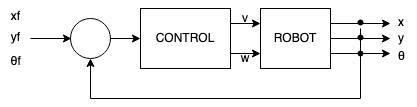
\includegraphics[scale=0.7]{graficos/bloque.png}
  \caption{Sistema de Control Lazo Cerrado}
\end{figure}


\[\dot{x} = v cos \Theta \qquad \dot{y} = v sin \Theta \dot{\Theta} = \omega \]

Un vector de error compuesto por una distancia \textbf{a} y un ángulo \textbf{$\alpha$} 

\begin{figure}[h]
  \centering
  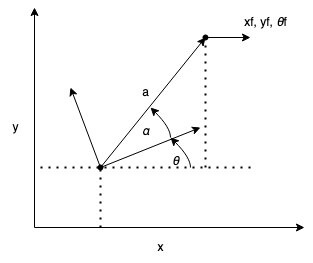
\includegraphics[scale=0.7]{graficos/grafico.png}
  \caption{Sistema}
\end{figure}

podemos ver $\Theta_{error}$ como: \\
\[ \Theta_{error} = \Theta + \alpha = tg \frac{ye}{xe} \]

consideramos nuestro vector de error:

\[ a = \sqrt{(xf-x)^{2}+(yf-y)^2} = \sqrt{x_{error}^{2} + y_{error}^2} \]

\[ \alpha = tg^{-1} \frac{y_{error}}{x_{error}} - \Theta\]

\textbf{Dinámica del error} $\dot{a}$, $\dot{\alpha}$ en función de v, w

\[ a = (x_{e}^{2} + y_{e}^{2})^{\frac{1}{2}}\]

\[ \dot{a} = \frac{\partial a}{\partial x_{error}}*\dot{x_{error}} + \frac{\partial a}{\partial y_{error}}*\dot{y_{error}}\]

\[ = \frac{1}{2} (x_{error}^{2} + y_{error}^{2})^{-\frac{1}{2}}*(2x_{error})*\dot{x_{error}} + \frac{1}{2} (x_{error}^{2}+y_{error}^2)^{-\frac{1}{2}}(2y_{error})*\dot{y_{error}}\]

\section{Resultados}


%------------------------------------------------
\section{Conclusiones}


%----------------------------------------------------------------------------------------
%	REFERENCE LIST
%----------------------------------------------------------------------------------------

\begin{thebibliography}{2} % Bibliography - this is intentionally simple in this template

\bibitem{Boney96} Boney, L., Tewfik, A.H., and Hamdy, K.N., ``Digital
  Watermarks for Audio Signals," \emph{Proceedings of the Third IEEE
    International Conference on Multimedia}, pp. 473-480, June 1996.
\bibitem{MG} Goossens, M., Mittelbach, F., Samarin, \emph{A LaTeX
  Companion}, Addison-Wesley, Reading, MA, 1994.
\bibitem{HK} Kopka, H., Daly P.W., \emph{A Guide to LaTeX},
  Addison-Wesley, Reading, MA, 1999.
\bibitem{Pan} Pan, D., ``A Tutorial on MPEG/Audio Compression," \emph{IEEE
  Multimedia}, Vol.2, pp.60-74, Summer 1998.
  
\end{thebibliography}

%----------------------------------------------------------------------------------------

\end{document}
